\documentclass[12pt]{article}
\usepackage{sbc-template}
\usepackage{graphicx}
\usepackage{amsmath}
%\usepackage{subfigure}
%\usepackage{times,amsmath,epsfig}
%\usepackage{graphicx,url}
 \makeatletter
 \newif\if@restonecol
 \makeatother
 \let\algorithm\relax
 \let\endalgorithm\relax 
\usepackage[lined,algonl,ruled]{algorithm2e}
\usepackage{multirow}
\usepackage[brazil]{babel}
\usepackage[utf8]{inputenc}  

\sloppy

\title{TRABALHO PRÁTICO 3: \\ Expansor de Macros}

\author{Pedro Lopes Miranda Junior}

\address{Departamento de Ciência da Computação -- Universidade Federal de Minas Gerais (UFMG)
\email{plmj@dcc.ufmg.br}
}

\begin{document}
\maketitle

\begin{resumo}
 Este documento tem por objetivo descrever um expansor de
 macros que será usado durante a diciplina de Software Básico a fim de realizar
 experimentos em uma máquina virtual com base nos conceitos teóricos vistos.
\end{resumo}

\section{Introdução}
\label{introducao}
Ao longo do curso serão estudados diversos conceitos sobre liguagem de máquina.
Perante isso, serão dados diversos trabalhos que testarão alguns dos inúmeros
conceitos abordados.

Após a implementação de uma máquina virtual e de um montador é necessário um
expansor de macros que expanda e substitua as chamadas de macros pelo código
inserido entre as pseudo-instruções BEGINMACRO e ENDMACRO. Uma macro deve
receber um nome que é usado para identifica-la.

Para isso é necessário ler o arquivo de entrada, que contem as macros, duas
vezes. Na primeira há a construção da tabela de macros. Na segunda a
substituição da macro pelo trecho de código é feita.

Abaixo será apresentada a solução proposta bem como os testes e decisões de
implementação.

\section{Solução Proposta}
\label{solucao_proposta}

Para solucionar o problema, foi criada uma estrutura de dados chamada
macro\_t a tabela de macros.
Esta tabela guarda o nome, o código e o parametro da macro, caso ela apresente.

O programa expansor foi criado em duas funções que percorrem o arquivo de
entrada com o código fonte duas vezes. As funções estão explicadas abaixo.
\subsection{Algoritmos}

Foram implementadas algumas funções que auxiliam no funcionamento do expansor, 
portanto todas as funções operam sobre o tipo macro\_t.
\newpage

\subsubsection{Funções}
\begin{algorithm}[h!]
\begin{footnotesize}
   \textbf{firs\_tstep;} \textit{Faz a primeira passagem sobre o código fonte
   criando a tabela de macros.} \\
   \textbf{second\_step;} \textit{Faz a segunda passagem sobre o código fonte
   substituindo as chamdas de macro pelo código inserido na mesma. Além disso
   faz o tratamento de macros com parâmetro e de labels internas a macro.} \\
\caption{Funções do expansor}
\end{footnotesize}
\end{algorithm}


\section{Implementação}
\label{implementacao}
Na implementação do problema proposto foram tomadas várias decisões, dentre
elas criar um tipo de dados para o expansor, dividir o código em funções
de modo que na função principal fique o menor conteúdo possível ajudando no
encapsulamento do código e em futuras manutenções e melhorias, além do fato de
usar a linguagem C++ e seus recursos extras em relação a linguagem C, utilizada
nos trabalhos anteriores.

Foi decidido criar um tipo de dados para a macro pois esse tipo de
disposição facilita a adição futura de demais estruturas caso necessário.
Além disso o acesso ao TAD é feito de maneira melhor estruturada e o
encapsulamento é melhor feito.

A divisão do código em funções ajuda no encapsulamento do TAD, e na melhor
modularização do mesmo.

\subsection{Código}
O código foi dividido em arquivos \textit{.cpp} e \textit{.h} que estão listados
abaixo

\subsubsection{Arquivos .cpp}
\begin{itemize}
\item \textbf{main.cpp:} Contém a função principal do expansor;
\item \textbf{expansor.cpp:} Contém as funções do tipo macro;
\end{itemize}

\subsubsection{Arquivos .h}

\begin{itemize}
\item \textbf{expansor.h:} Contém as definições das funções do tipo macro
\end{itemize}

\subsection{Compilação}

O programa deve ser compilado através de um makefile, chamando
\textit{expansor}
ou através do compilador GCC chamando:\\

\begin{footnotesize}
\begin{verbatim} gpp -Wall main.cpp expansor.cpp -o expansor \end{verbatim}
\end{footnotesize}

\subsection{Execução}

Para a execução do programa deverão ser recebidos,impreterívelmente, o nome do 
arquivo com o código assembly a ser executado e o arquivo de saída. 

O comando para execução do programa é da forma: \\

\begin{footnotesize}
\begin{verbatim} ./expansor <entrada> <saída> \end{verbatim}
\end{footnotesize}

\subsubsection{Formato da entrada}
O arquivo de entrada citado deverá ser um programa em linguagem assembly,
onde cada linha conterá uma instrução, podendo ou não ter uma macro.

\subsubsection{Formato da saída}
O programa imprimirá no arquivo de saída o código também no assembly
característico, porém com as macros expandidas.

\section{Avaliação Experimental}
\label{avaliacao_experimenta}
O programa foi executado e testado numa máquina rodando o sistema baseado em
debian Linux Mint. A máquina em questão tem uma memória de 8GB e um processador
Core I7 de 2.2GHz.

Foram feitos vários testes de execução do programa,onde todas as funções
testadas funcionaram de maneira rápida e sem erro. Abaixo apresentamos imagens
da execução do programa e sua saída.

\begin{figure}[h!]
\centering
 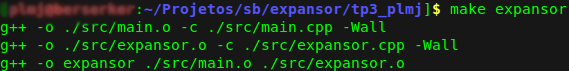
\includegraphics[scale=0.5]{./img/make.png}
 \caption{Comando Make}
\end{figure}

\begin{figure}[h!]
\centering
 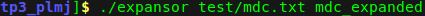
\includegraphics[scale=0.5]{./img/exec.png}
   \caption{Comando de execução do programa}
\end{figure}

\newpage

\begin{figure}[h!]
\centering
 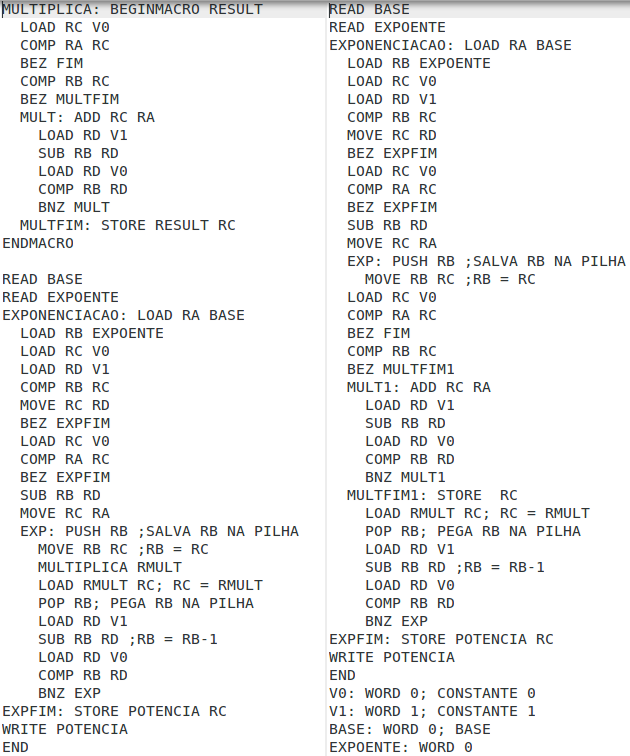
\includegraphics[scale=0.5]{./img/teste.png}
 \caption{Saída exemplos de programas normal e já expandido}
\end{figure}

\section{Conclusão}
\label{conclusao}
O trabalho correu sem grandes problemas, sendo a parte mais difícil a criação
dos progrmas de testes, pois montar alguns daqueles códigos em asembly é
extremamente difícil.

O programa atendeu a diversos valores de entrada e creio que a solução proposta
atenda ao especificado

\end{document}
